\documentclass{article}

% see readme
\def\OPTIONConf{1}%
\usepackage{joshuadunfield}
\usepackage{llproof}
% !TEX root = hazelnut-popl17.tex

% Violet hotdogs; highlight color helps distinguish them
\newcommand{\llparenthesiscolor}{\textcolor{violet}{\llparenthesis}}
\newcommand{\rrparenthesiscolor}{\textcolor{violet}{\rrparenthesis}}

% HTyp and HExp
\newcommand{\hcomplete}[1]{#1~\mathsf{complete}}

% HTyp
\newcommand{\htau}{\dot{\tau}}
\newcommand{\tarr}[2]{\inparens{#1 \rightarrow #2}}
\newcommand{\tarrnp}[2]{#1 \rightarrow #2}
\newcommand{\tnum}{\mathtt{num}}
\newcommand{\tehole}{\llparenthesiscolor\rrparenthesiscolor}
\newcommand{\tsum}[2]{\inparens{{#1} + {#2}}}

\newcommand{\tcompat}[2]{#1 \sim #2}
\newcommand{\tincompat}[2]{#1 \nsim #2}

% HExp
\newcommand{\hexp}{\dot{e}}
\newcommand{\hlam}[2]{\inparens{\lambda #1.#2}}
\newcommand{\hap}[2]{#1(#2)}
\newcommand{\hapP}[2]{(#1)~(#2)} % Extra paren around function term
\newcommand{\hnum}[1]{\underline{#1}}
\newcommand{\hadd}[2]{\inparens{#1 + #2}}
\newcommand{\hehole}{\llparenthesiscolor\rrparenthesiscolor}
\newcommand{\hhole}[1]{\llparenthesiscolor#1\rrparenthesiscolor}
\newcommand{\hindet}[1]{\lceil#1\rceil}
\newcommand{\hinj}[2]{\mathtt{inj}_{#1}({#2})}
\newcommand{\hcase}[5]{\mathtt{case}({#1},{#2}.{#3},{#4}.{#5})}

\newcommand{\hGamma}{\dot{\Gamma}}
\newcommand{\domof}[1]{\text{dom}(#1)}
\newcommand{\hsyn}[3]{#1 \vdash #2 \Rightarrow #3}
\newcommand{\hana}[3]{#1 \vdash #2 \Leftarrow #3}

% ZTyp and ZExp
\newcommand{\zlsel}[1]{{\bowtie}{#1}}
\newcommand{\zrsel}[1]{{#1}{\bowtie}}
\newcommand{\zwsel}[1]{
  \setlength{\fboxsep}{0pt}
  \colorbox{green!10!white!100}{
    \ensuremath{{{\textcolor{Green}{{\hspace{-2px}\triangleright}}}}{#1}{\textcolor{Green}{\triangleleft{\vphantom{\tehole}}}}}}
}

\newcommand{\removeSel}[1]{#1^{\diamond}}

% ZTyp
\newcommand{\ztau}{\hat{\tau}}

% ZExp
\newcommand{\zexp}{\hat{e}}

% Direction
\newcommand{\dParent}{\mathtt{parent}}
\newcommand{\dChildn}[1]{\mathtt{child}~\mathtt{{#1}}}
\newcommand{\dChildnm}[1]{\mathtt{child}~{#1}}

% Action
\newcommand{\aMove}[1]{\mathtt{move}~#1}
	\newcommand{\zrightmost}[1]{\mathsf{rightmost}(#1)}
	\newcommand{\zleftmost}[1]{\mathsf{leftmost}(#1)}
\newcommand{\aSelect}[1]{\mathtt{sel}~#1}
\newcommand{\aDel}{\mathtt{del}}
\newcommand{\aReplace}[1]{\mathtt{replace}~#1}
\newcommand{\aConstruct}[1]{\mathtt{construct}~#1}
\newcommand{\aConstructx}[1]{#1}
\newcommand{\aFinish}{\mathtt{finish}}

\newcommand{\performAna}[5]{#1 \vdash #2 \xlongrightarrow{#4} #5 \Leftarrow #3}
\newcommand{\performAnaI}[5]{#1 \vdash #2 \xlongrightarrow{#4}\hspace{-3px}{}^{*}~ #5 \Leftarrow #3}
\newcommand{\performSyn}[6]{#1 \vdash #2 \Rightarrow #3 \xlongrightarrow{#4} #5 \Rightarrow #6}
\newcommand{\performSynI}[6]{#1 \vdash #2 \Rightarrow #3 \xlongrightarrow{#4}\hspace{-3px}{}^{*}~ #5 \Rightarrow #6}
\newcommand{\performTyp}[3]{#1 \xlongrightarrow{#2} #3}
\newcommand{\performTypI}[3]{#1 \xlongrightarrow{#2}\hspace{-3px}{}^{*}~#3}

\newcommand{\performMove}[3]{#1 \xlongrightarrow{#2} #3}
\newcommand{\performDel}[2]{#1 \xlongrightarrow{\aDel} #2}

% Form
\newcommand{\farr}{\mathtt{arrow}}
\newcommand{\fnum}{\mathtt{num}}
\newcommand{\fsum}{\mathtt{sum}}

\newcommand{\fasc}{\mathtt{asc}}
\newcommand{\fvar}[1]{\mathtt{var}~#1}
\newcommand{\flam}[1]{\mathtt{lam}~#1}
\newcommand{\fap}{\mathtt{ap}}
% \newcommand{\farg}{\mathtt{arg}}
\newcommand{\fnumlit}[1]{\mathtt{lit}~#1}
\newcommand{\fplus}{\mathtt{plus}}
\newcommand{\fhole}{\mathtt{hole}}
\newcommand{\fnehole}{\mathtt{nehole}}

\newcommand{\finj}[1]{\mathtt{inj}~#1}
\newcommand{\fcase}[2]{\mathtt{case}~#1~#2}

% Talk about formal rules in example
\newcommand{\refrule}[1]{\textrm{Rule~(#1)}}

\newcommand{\herase}[1]{\left|#1\right|_\textsf{erase}}

\newcommand{\arrmatch}[2]{#1 \blacktriangleright_{\rightarrow} #2}


\newcommand{\TABperformAna}[5]{#1 \vdash & #2                & \xlongrightarrow{#4} & #5 & \Leftarrow #3}
\newcommand{\TABperformSyn}[6]{#1 \vdash & #2 \Rightarrow #3 & \xlongrightarrow{#4} & #5 \Rightarrow #6}
\newcommand{\TABperformTyp}[3]{& #1 & \xlongrightarrow{#2} & #3}

\newcommand{\TABperformMove}[3]{#1 & \xlongrightarrow{#2} & #3}
\newcommand{\TABperformDel}[2]{#1 \xlongrightarrow{\aDel} #2}

\newcommand{\sumhasmatched}[2]{#1 \mathrel{\textcolor{black}{\blacktriangleright_{+}}} #2}

\newcommand{\subminsyn}[1]{\mathsf{submin}_{\Rightarrow}(#1)}
\newcommand{\subminana}[1]{\mathsf{submin}_{\Leftarrow}(#1)}


\newcommand{\inparens}[1]{{\color{gray}(}#1{\color{gray})}}

%% rule names for appendix
\newcommand{\rname}[1]{\textsc{#1}}
\newcommand{\gap}{\vspace{7pt}}

% for header page
\newcommand{\vs}{\vspace{20pt}}

% for header page
\newcommand{\pt}[1]{\MakeUppercase{
    \centering{}
    \large{}
    #1 \\
    \vs{}
  }}

% allow custom lexer for pygmentize
% https://github.com/gpoore/minted/issues/176#issuecomment-695344998
\usepackage{minted}
\usepackage{regexpatch}

\makeatletter
\newcommand{\minted@def@optcl@novalue}[2]{%
  \define@key{minted@opt@g}{#1}[]{%
    \minted@addto@optlistcl{\minted@optlistcl@g}{#2}%
    \@namedef{minted@opt@g:#1}{#2}}%
  \define@key{minted@opt@g@i}{#1}[]{%
    \minted@addto@optlistcl{\minted@optlistcl@g@i}{#2}%
    \@namedef{minted@opt@g@i:#1}{#2}}%
  \define@key{minted@opt@lang}{#1}[]{%
    \minted@addto@optlistcl@lang{minted@optlistcl@lang\minted@lang}{#2}%
    \@namedef{minted@opt@lang\minted@lang:#1}{#2}}%
  \define@key{minted@opt@lang@i}{#1}[]{%
    \minted@addto@optlistcl@lang{%
      minted@optlistcl@lang\minted@lang @i}{#2}%
    \@namedef{minted@opt@lang\minted@lang @i:#1}{#2}}%
  \define@key{minted@opt@cmd}{#1}[]{%
    \minted@addto@optlistcl{\minted@optlistcl@cmd}{#2}%
    \@namedef{minted@opt@cmd:#1}{#2}}%
}

% new minted option "custom" for adding command line option "-x"
\minted@def@optcl@novalue{custom}{-x}

% new minted option "formatter=<formatter>" for specifying pygments formatter
\minted@def@opt{formatter}

% apply "-f <formatter>"
\newcommand\minted@formatter{%
  \minted@get@opt{formatter}{latex}\space
}

% Note: may require fix to regexpatch:
% https://tex.stackexchange.com/questions/578518/regexpatchcmd-failing-with-latex2e-2020-10-01-patch-level-4-use-cs-replacemen#comment1469403_578518
\xpatchcmd*\minted@checkstyle
  {-f latex }
  {-f \minted@formatter}
  {}{\fail}
\xpatchcmd*\minted@pygmentize
  {-f latex }
  {-f \minted@formatter}
  {}{\fail}

  \makeatother
  % end custom lexer for pygmatize

% Need VerbatimEnvironment:
% https://tex.stackexchange.com/a/400115
\newenvironment{hminted}
{\VerbatimEnvironment
\begin{minted}[escapeinside=//,frame=single,custom]{../latex-includes/hazel_lexer.py:HazelLexer}}
{\end{minted}}

% hazel inline; don't really know what's going on here
% https://tex.stackexchange.com/a/181393
\newcommand{\hmintinlinet}{
  \mintinline[escapeinside=//,frame=single,custom]{../latex-includes/hazel_lexer.py:HazelLexer}
}
\newcommand{\hmintinline}[1]{\expandafter\hmintinlinet\expandafter{#1}}

% \newcommand{\ab}{expanded stuff}
% \newcommand{\pythoninline}{\mintinline[]{python}}

% hazel inputminted
\newcommand{\inputhminted}[1]{\inputminted[escapeinside=//,frame=single,custom]{../latex-includes/hazel_lexer.py:HazelLexer}{lstings/#1.hz}}

% ocaml inputminted
\newcommand{\inputominted}[1]{\inputminted[escapeinside=//,frame=single]{ocaml}{lstings/#1.ml}}


% extra math operators
% especially for math operators that are introduced in this paper, want to
% declare them here so they are easily changeable
\DeclareMathOperator{\fix}{fix}       % fixpoint
\newcommand{\env}{\sigma}             % environment
\newcommand{\pp}{\Uparrow}            % post-process
\newcommand{\pplc}{\pp_{[]}}          % post-process lambda conversion (substitution) operator
\newcommand{\pplco}{\pp_{[],1}}       % post-process lc part 1
\newcommand{\pplct}{\pp_{[],2}}       % post-process lc part 2
\newcommand{\ppn}{\pp_{i}}            % post-process hole closure numbering
\newcommand{\ppnd}{\pp_{i,d}}         % post-process hole closure numbering (results only)
\newcommand{\ppns}{\pp_{i,\env}}      % post-process hole closure numbering (sigmas only)
\newcommand{\pplcl}{PPI$_{[]}$}       % post-process lambda within evaluation boundary conversion label
\newcommand{\pplclo}{PPO$_{[]}$}      % post-process lambda outside evaluation boundary conversion label
\newcommand{\ppndl}{PP$_{i,d}$}       % post-process hole closure numbering label
\newcommand{\ppnsl}{PP$_{i,\env}$}     % post-process hole closure numbering label
\newcommand{\pth}{p}                  % path
\newcommand{\hci}{H}                  % hole instance/closure info
\DeclareMathOperator{\hid}{hid}       % hole instance id generator

% for use in Hazel listings
\newcommand{\rar}{$\rightarrow$}
\newcommand{\Rar}{$\Rightarrow$}
\newcommand{\lbd}{$\lambda$}
\newcommand{\heh}[1]{$\hehole^{#1}$}

% for missing references
\newcommand{\todo}[1]{\textbf{[TODO: #1]}}
\newcommand{\todoref}[1]{\textbf{[TODO: need reference(s): #1]}}

%%% Local Variables:
%%% mode: latex
%%% TeX-master: "../thesis/main"
%%% End:


\usepackage{amsmath}
\usepackage{amssymb}
\usepackage{stmaryrd}
\usepackage{hyperref}
\usepackage{minted}
\usepackage{geometry}
\usepackage{setspace}

% https://tex.stackexchange.com/a/55088
\makeatletter{}
\renewcommand\tableofcontents{%
  \@starttoc{toc}%
}
\renewcommand\listoffigures{%
  \@starttoc{lof}%
}
\makeatother{}

% https://tex.stackexchange.com/a/132647
\usepackage{etoolbox}
\patchcmd{\thebibliography}{\section*{\refname}}{}{}{}

\begin{document}

\doublespacing
\pagenumbering{roman}

% title and signature pages
\thispagestyle{empty}

{
  \centering
  \large

  \pt{
    The Cooper Union for the Advancement of Science and Art \\
    Albert Nerken School of Engineering
  }
  
  \vfill{}
  
  {
    {
      \huge
      Optimization by memoization of evaluation tasks \\
      in the Hazel structured programming environment \\
    }
    \vs{}
    by Jonathan Lam \\
  }

  \vfill{}

  {
    A thesis submitted in partial fulfillment of the requirements for the degree of \\
    Master of Engineering \\
  }

  \vfill{}

  {
    Professor Fred L. Fontaine, Advisor \\
    Professor Robert Marano, Co-advisor \\
    % TODO: Can I add Prof. Omar on the title page too?
  }


  \vfill{}
  {
    Performed in collaboration with the \\
    Future of Programming Lab at the University of Michigan \\
  }
}

%%% Local Variables:
%%% mode: latex
%%% TeX-master: "main"
%%% End:

\thispagestyle{empty}

{
  \pt{
    The Cooper Union for the Advancement of Science and Art \\
    Albert Nerken School of Engineering
  }
  
  \noindent{} This thesis was prepared under the direction of the Candidate's Thesis Advisor and has received approval. It was submitted to the Dean of the School of Engineering and the full Faculty, and was approved as partial fulfillment of the requirements for the degree of Master of Engineering.
}

\vfill{}

\begin{singlespace}
  \raggedleft{}
  \rule{0.5\textwidth}{1pt} \\
  \makebox[0.5\textwidth][r]{
    Barry L. Shoop, Ph.D., P.E. \hfill Date
  } \\
\end{singlespace}

\vfill{}

\begin{singlespace}
  \raggedright{}
  \rule{0.5\textwidth}{1pt} \\
  \makebox[0.5\textwidth][l]{
    Fred L. Fontaine, Ph.D. \hfill Date
  } \\
\end{singlespace}

\vfill{}
\vfill{}

%%% Local Variables:
%%% mode: latex
%%% TeX-master: "main"
%%% End:

\pt{Acknowledgments}

TODO

% Family, aunt/uncles/everyone i've lived with
% 10B
% Victor and Derek
% Advisor, UMich ppl

%%% Local Variables:
%%% mode: latex
%%% TeX-master: "main"
%%% End:

\pt{Abstract}

\noindent{}Hazel is a live programming environment with typed holes that serves as a reference implementation of Hazelnut Live dynamic semantics and the Hazelnut static semantics, both of which tackle the ``gap problem.'' This work attempts to further develop the Hazel evaluation model by implementing the environment model of evaluation (rather than the current substitution model) and memoizing several evaluation-related operations to improve performance. Additionally, we provide an implementation-level description and a reference implementation of the fill-and-resume (FAR) performance optimization proposed in Hazelnut Live. We produce a metatheory and reference implementation of the proposed changes. We also benchmark the our implementation against the existing Hazel implementation and show that the results match the expectation, although there is room for future improvement with further development of FAR. Finally, we discuss some useful theoretical generalizations that result from this work and how we hope this work informs future development on Hazel.

%%% Local Variables:
%%% mode: latex
%%% TeX-master: "main"
%%% End:


% toc and lof
\pt{Table of contents}
\tableofcontents{}
\clearpage{}
\pt{List of figures}
\listoffigures{}

% list of nomenclature/terminology/notation
\pt{List of notations}
% \FloatBarrier{}

% nomencl package is too confusing, just use manual tables

\newcommand{\colwidths}{p{4cm}p{10cm}}

\singlespacing

\begin{table}[H]
  \centering
  \begin{tabular}{\colwidths}
    \hline\hline
    $e$ & (External) expression \\
    $\tau$ & Type \\
    $\Gamma$ & Typing context \\
    $\Delta$ & Hole context \\
    $\Gamma\vdash e:\tau$ & Type judgment \\
    $\Gamma\vdash e\Rightarrow\tau$ & Synthetic type judgment \\
    $\Gamma\vdash e\Leftarrow\tau$ & Analytic type judgment \\
    $[e'/x]e$ & Substitution of $e'$ for $x$ in $e$ \\
    \hline\hline
  \end{tabular}
  \caption{Common notation for the $\lambda$-calculus}
  \label{tab:symb_general}
\end{table}

\begin{table}[H]
  \centering
  \begin{tabular}{\colwidths}
    \hline\hline
    \ulc & Untyped $\lambda$-calculus \\
    \stlc & Simply-typed $\lambda$-calculus \\
    \gtlc & Gradually-typed $\lambda$-calculus \\
    $\Lambda_{\rightarrow}^{\tehole}$ & $\lambda$-calculus with typed holes \\
    \hline\hline
  \end{tabular}
  \caption{The $\lambda$-calculi}
  \label{tab:symb_general}
\end{table}

\begin{table}[H]
  \centering
  \begin{tabular}{\colwidths}
    \hline\hline
    $\gtlch$ & Unknown type \\
    $\tau\sim\tau'$ & Type consistency \\
    $\arrmatch{\tau}{\tau_1\to\tau_2}$ & Matched arrow judgment \\
    $\Gamma\vdash e\leadsto d:\tau$ & Elaboration judgment \\
    $d\langle\tau\Rightarrow\tau'\rangle$ & Cast expression \\
    \hline\hline
  \end{tabular}
  \caption{The gradually-typed $\lambda$-calculus}
  \label{tab:symb_general}
\end{table}

\begin{table}[H]
  \centering
  \begin{tabular}{\colwidths}
    \hline\hline
    $d$ & Internal expression \\
    $\lambda x:\tau.d$ & $\lambda$-abstraction \\
    $\fix f:\tau.d$ & Fixpoint form \\
    $\env$ & Environment \\
    $x,f$ & Variable name \\
    $u$ & Hole number \\
    $i$ & Hole instance or closure number \\
    $\hehole^{u:i}$ & Empty hole expression \\
    $\hhole{d}^{u:i}$ & Non-empty hole expression \\
    $[\env]d$ & Generalized closure \\
    \hline\hline
  \end{tabular}
  \caption{Hazel internal language}
  \label{tab:symb_hazel_dhexp}
\end{table}

\begin{table}[H]
  \centering
  \begin{tabular}{\colwidths}
    \hline\hline
    $d\textsf{ value}$ & Value \\
    $d\textsf{ final}$ & Final \\
    $\env\vdash d\Downarrow d'$ & Evaluation \\
    \hline\hline
  \end{tabular}
  \caption{Hazel evaluation judgments}
  \label{tab:symb_hazel_dhexp}
\end{table}

\begin{table}[H]
  \centering
  \begin{tabular}{\colwidths}
    \hline\hline
    $\hci$ & Hole instance/closure information \\
    $\hid$ & Hole instance/closure id generation function \\
    $\pth$ & Hole closure parent \\
    $d\pp d'$ & Postprocessing \\
    $d\pplc d'$ & Postprocessing ($\lambda$-conversion) \\
    $\hci,\pth\vdash d\ppn d'\dashv\hci'$ & Postprocessing (hole closure numbering) \\
    \hline\hline
  \end{tabular}
  \caption{Hazel postprocessing judgments}
  \label{tab:symb_hazel_dhexp}
\end{table}

\begin{table}[H]
  \centering
  \begin{tabular}{\colwidths}
    \hline\hline
    $\nodiff{d_1}{d_2}$ & No diff (empty diff) between $d_1$ and $d_2$ \\
    $\nfdiff{d_1}{d_2}$ & Non-fill diff from $d_1$ to $d_2$ \\
    $\fdiff{d_1}{d_2}{u}{d}$ & Fill diff from $d_1$ to $d_2$ with fill parameters $u$ and $d$ \\
    $\sdiff{d_1}{d_2}{u}{d}$ & Some (non-empty) diff from $d_1$ to $d_2$ \\
    $\adiff{d_1}{d_2}{u}{d}$ & Any (possibly empty) diff from $d_1$ to $d_2$ \\
    $d_1\sim d_2$ & Expression form equality \\
    \hline\hline
  \end{tabular}
  \caption{Fill-and-resume structural diff algorithm}
  \label{tab:symb_far-diff}
\end{table}

\begin{table}[H]
  \centering
  \begin{tabular}{\colwidths}
    \hline\hline
    $\far{u}{d}{d'}=d''$ & Fill-and-resume operation on an expression \\
    $\far{u}{d}{\env}=\env'$ & Fill-and-resume operation on an environment \\
    $\llbracket\env\rrbracket d$ & Closure with re-eval flag set \\
    $\hhole{d}_i$ & Expression $d$ filled in hole with hole closure number $i$ \\
    $\fenv$ & Fill memoization context\\
    $\env,\fenv\vdash d\Downarrow d'\dashv\fenv'$ & Fill-memoized evaluation \\
    \hline\hline
  \end{tabular}
  \caption{Fill-and-resume pre-processing and evaluation}
  \label{tab:symb_far-eval}
\end{table}

\doublespacing

%%% Local Variables:
%%% mode: latex
%%% TeX-master: "main"
%%% End:


% end front matter
\pagenumbering{arabic}
\clearpage{}

\chapter{Introduction}
\label{sec:introduction}

\section{Problem statement}
\label{sec:prob_stmt}

\begin{figure}
  \centering
  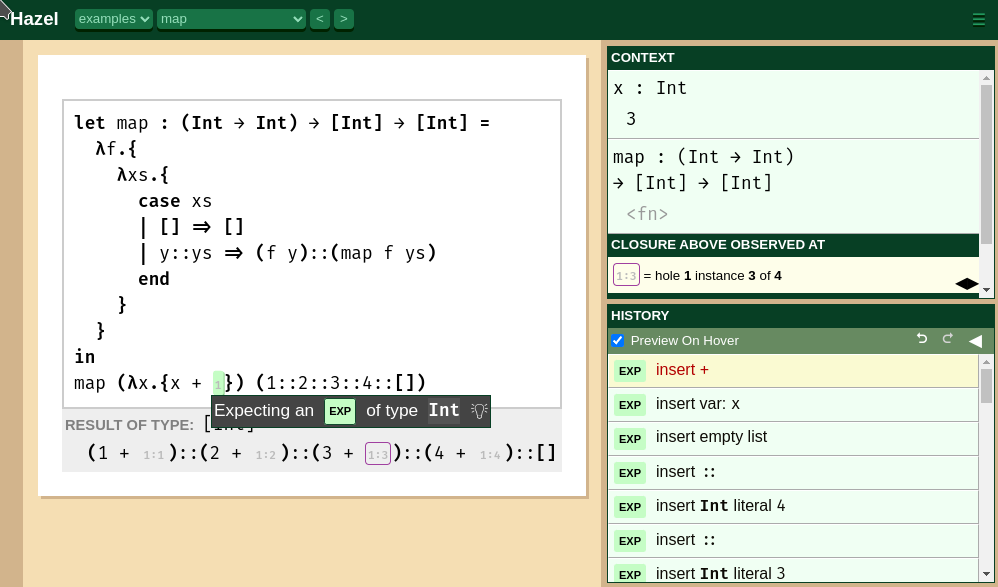
\includegraphics[width=4in]{img/hazel_ui.png}
  \caption[Screenshot of the Hazel live programming environment.]{A screenshot of the Hazel live programming environment. Screenshot taken of the dev branch demo on 02/06/2022 \cite{HazelDemo2022}.}
  \label{fig:screenshot-hazel-ui}
\end{figure}

Unstructured plaintext editing has remained the dominant mode of programming for decades, but makes it more difficult to implement editor services to aid the process. Structural editors, on the other hand, only allow valid edit states. Several structural editors, such as Scratch \cite{maloney2010scratch}, Lamdu \cite{lotem_chuchem}, and mbeddr \cite{voelter2012mbeddr}, have been proposed to improve the programming experience and introduce editor services, such as the elimination of syntax errors or graphical editing.

Hazel \cite{hazel_git} is an experimental structural language definition and implementation that aims to solve the ``gap problem'': spatial and temporal holes that temporarily prevent code from being able to be compiled or evaluated. The structural editor is defined by a bidirectional edit calculus Hazelnut \cite{conf/popl/Hazelnut17}, which governs the structural editor and the static semantics (typing rules) of the language. The dynamic semantics (evaluation semantics) are described in Hazelnut Live \cite{conf/popl/HazelnutLive19}.

Hazel is a relatively new research effort by the University of Michigan's Future of Programming Lab (FPLab), with little effort placed on performance optimizations. This work attempts to achieve several enhancements to Hazelnut Live that will benefit the performance of evaluation and related tasks. Part of the work will be focused on transitioning the evaluation model from using substitution for variable bindings to using environments, with emphasis on evaluation of holes and postprocessing of the evaluation result to match the result from evaluation with substitution. The latter parts of this work will use the environment model of evaluation to improve the memoization of certain tasks specific to Hazel (such as hole closure numbering), and also implement the fill-and-resume performance enhancement described in \cite{conf/popl/HazelnutLive19}. The novelty of this work lies in the optimization capacity in the unique design of the Hazel language as a live programming editor with expression holes.

\section{The contribution of this work}
\label{sec:contribution}

This thesis presents several algorithms designed for Hazel's evaluation. These algorithms are provided using the big-step inference semantics notation introduced in \cref{sec:semantics-notation}.

Firstly, we provide the evaluation semantics of the Hazel language using the environment model. We aim to keep the implementation pure, introduce uniquely-numbered environments (for later use in memoization), and describe the evaluation of holes (which are unique to Hazel). We introduce the concepts of generalized closures, and the evaluation boundary.

Secondly, we describe the postprocessing algorithm, which is mostly memoized by environments and has the two major functions. The first is to convert the result to the equivalent result if substitution was used. The second is to number hole closure instances.

Lastly, we develop the fill-and-resume process, as originally proposed (but not implemented) in \cite{conf/popl/HazelnutLive19}. We provide a possible implementation, including an algorithm to detect a valid fill operation and advice on memoizing the resumption operation.

The performance of this work is measured primarily in terms of empirical performance gains (via evaluation-step counting and benchmarking), and discussed with respect to the theoretical performance. Hazelnut \cite{conf/popl/Hazelnut17} and Hazelnut Live \cite{conf/popl/HazelnutLive19} mechanize proofs of their work using the Agda interactive proof checker. We do not provide mechanized proofs of our work; instead, we provide a series of core metatheorems describing invariants describing Hazel evaluation, and argue the correctness of these metatheorems by informal reasoning on the provided inference rules. A mechanized proof using Agda is deferred for future work.

\section{Structural overview}
\label{sec:structural_overview}

\Cref{sec:prog_lang_principles} provides a background on necessary topics in programming language (PL) theory and programming language implementations, in order to frame the understanding for the Hazel live programming environment. \Cref{sec:hazel} provides an overview of Hazel, in order to frame the work completed for this thesis project. \Crefrange{sec:env_model_evaluation}{sec:far_impl} describe the primary work completed for this project, as described in \Cref{sec:contribution}. \Cref{sec:evaluation} comprises an emprical performance assessment of the work. \Cref{sec:discussion} is a discussion of theoretical results. \Cref{sec:future_work} describes unfinished work and future research directions. \Cref{sec:concl} concludes with a summary of findings and future work. The Appendices contain extra inference rules and selected source code snippets.

%%% Local Variables:
%%% mode: latex
%%% TeX-master: "main"
%%% End:

\chapter{An overview of the Hazel programming environment}
\label{sec:hazel}

Hazel is the reference implementation for the Hazelnut bidirectionally-typed action semantics and the Hazelnut Live dynamic semantics. It is intended to serve as a proof-of-concept of the semantics with static holes that attempt to mitigate the gap problem; however, the implementation is becoming increasingly practical with recent additions to the language. The reference implementation is an interpreter written in OCaml and transpiled to Javascript using the \mintinline{text}|js_of_ocaml| (JSOO) library \cite{vouillon2014bytecode} so that it may be run client-side in the browser. A screenshot of the reference implementation is shown in \Cref{fig:screenshot-hazel-ui} \cite{HazelDemo2022}. The source code may be found on GitHub \cite{Hazel2022}. Hazel may be characterized as a purely functional, statically-typed, bidirectionally-typed, strict-order evaluation, structured editor programming language.

\section{Motivation for Hazel}
\label{sec:hazel-motivation}

\subsection{The gap problem}
\label{sec:gap-problem}

Programming editor environments aim to provide feedback to a programmer in the form of editor services such as syntax highlighting or warnings using the LSP. Live programming environments aim to provide continuous static (static type error) and dynamic (run-time type error) feedback in real-time, allowing for rapid prototyping. However, over the course of the lifetime of a program, the program may enter many edit states when it is \textit{meaningless} (ill-formed or ill-typed).

Editor services can only assign static and dynamic meaning to programs that are statically well-typed and free of dynamic type errors. Some may deploy reduced ad hoc algorithms of meaningless edit states. This means that over the course of editing, the programmer experiences temporal gaps between moments of complete editor services. This is known as the \textit{gap problem} \cite{10.1145/2499370.2462170,conf/popl/HazelnutLive19}.

\subsection{An intuitive introduction to typed expression holes}
\label{sec:typed-holes}

Hazelnut and Hazelnut Live address the gap problem by defining a static and dynamic semantics, respectively, for a small functional programming language extended with typed holes. It is built on top of a \textit{structure editor}, which ensures that a program is always well-formed (syntactically correct) by disallowing invalid edit actions. The Hazelnut action semantics for typed holes ensures that a well-formed program is always well-typed. The Hazelnut Live dynamic semantics defines an encapsulated behavior for type errors, such that evaluation continues ``around'' and captures information about type errors in order to provide dynamic feedback to the programmer.

The Hazelnut Live paper provides the following intuitive understanding of holes.

\begin{displayquote}
  Empty holes stand for missing expressions or types, and non-empty holes operate as ``membranes''
around static type inconsistencies (i.e. they internalize the ``red underline'' that editors commonly display under a type inconsistency).
\end{displayquote}

We have already acknowledged the existence of type holes in dynamically-typed languages and in the \gtclc{}, in which type holes are represented by the type $\gtlch$. This allows unannotated expressions to statically type-check, with the possibility of running into a dynamic type error at runtime.

Some languages also have the concept of expression holes, which allow a program to be well-typed with missing expressions. In Haskell, for example, the special error value \mintinline{haskell}|undefined| always type-checks but will immediately crash the program if it is encountered during evaluation. Haskell also provides the syntax \mintinline{haskell}|_u| for expression holes \todoref{cite this}, which provides static type information but will not successfully compile. The mechanism to insert expressions holes may be either automatic or manual \todoref{cite this}. However, no such example of expression holes have a well-defined dynamic semantics that allows continuation past the hole with useful feedback \todoref{cite this -- perhaps cite hazelnut 2019 paper}.

In summary, Hazel provides empty type and expression holes, which represent dynamic typing and missing expressions. Nonempty holes are also provided to encapsulate error conditions and provide a well-defined dynamic semantics while providing useful feedback to the user. The dynamic semantics is carefully defined to stop when such indeterminate expressions are encountered, but continue elsewhere (``around'' holes or failed casts) if possible.

\subsection{The Hazel interface}
\label{sec:hazel-interface}

In \Cref{fig:hazel-interface} the web interface for the Hazel live environment is shown. The left panel marked (1) is a informational panel showing the list of keyboard shortcuts to perform actions. Since Hazel is a structured editor, simply typing the program as plaintext will not work; one must use the appropriate shortcuts the construct and edit the program. (2) is the code view. Below the code, a gray box indicates the result of evaluating the expression. The program result updates in real time with every edit action, assuming that evaluation is turned on. (3) is the context inspector, which shows information about a hole if a hole is selected. It shows the hole environment and typing context, followed by the path to the hole and the number of hole instances. In this case, the third hole in the result is selected, in which $x$ has value $3$. Lastly, (4) shows a history of the edit actions. Hovering or clicking on a past edit state will revert the program to that edit state.

\begin{figure}
  \centering
  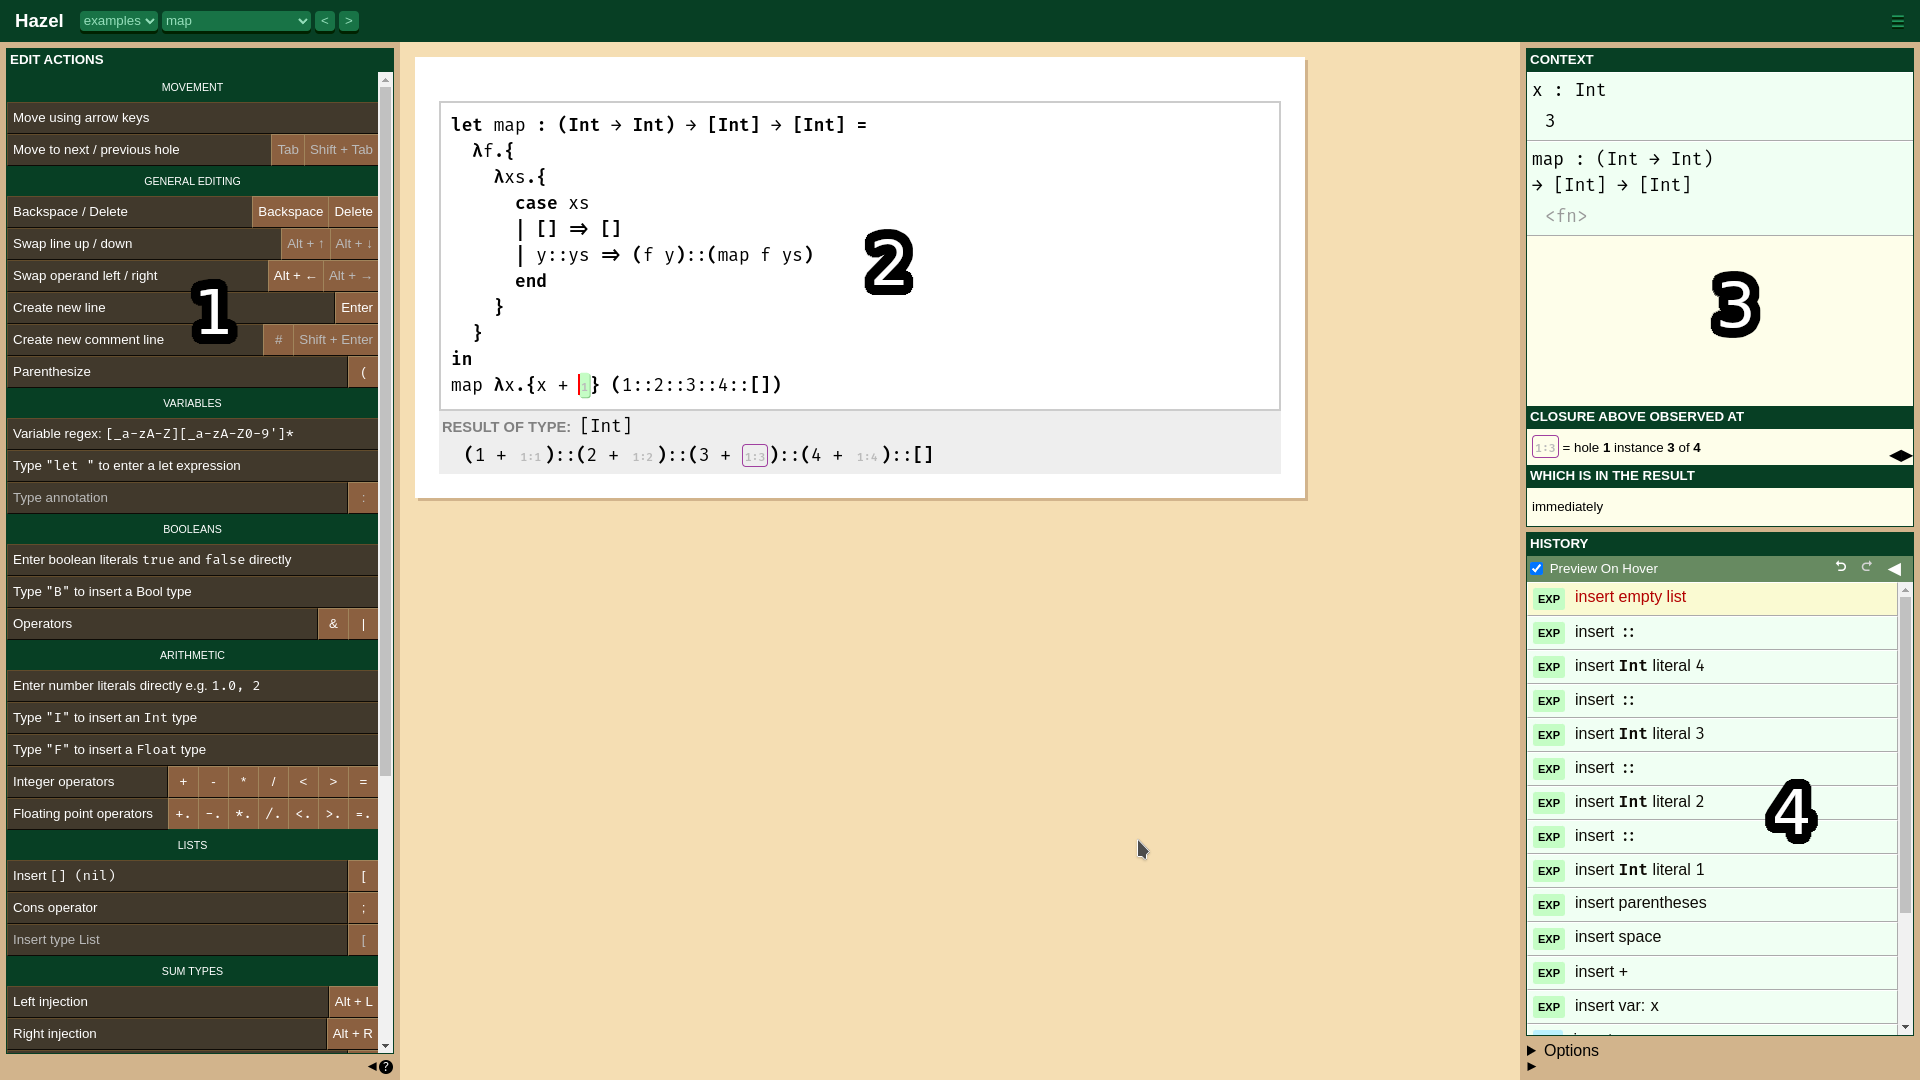
\includegraphics[width=\linewidth]{img/hazel_ui_annot.png}
  \caption{The Hazel interface, annotated}
  \label{fig:hazel-interface}
\end{figure}

\subsection{Implications of Hazel}
\label{sec:hazel-implications}

The main proposed use case of Hazel is its use in programming education, particularly for teaching functional programming, as it provides much useful feedback to the programmer for error conditions, allowing them to focus instead on semantic errors in their algorithm. This is being explored with the Hazel Tutor project \cite{potter2020hazel}.

Another research direction is in its use as a structural and graphical editor. For example, live GUIs \cite{omar2021filling} are being explored to enhance the editing experience by providing live, compositional, graphical interfaces, in addition to the benefits that Hazel's core calculi provide.

The result of a Hazel evaluation may contain holes, and thus not be fully evaluated. The Hazelnut Live paper \cite{conf/popl/HazelnutLive19} suggests the idea of hole-filling: since each hole in the result contains its lexical environment, we may ``resume'' evaluation without restarting evaluation from the beginning if a hole is filled -- this property is similar to that of computational notebooks. The problem with notebook execution is that it is stateful and running operations out-of-order may cause irreversible state changes that cause irreproducible results. On the other hand, resuming an evalution with fill-and-resume will produce the same result as if the program was run ordinarily from start to finish\footnote{This is a property known as \textit{commutativity} and described in \cite{conf/popl/HazelnutLive19}.} while avoiding re-evaluation of previous sections.

\section{Introduction to OCaml and Reason syntax}
\label{sec:ocaml-intro}

Previously, we have been introducing concepts using a pseudo-mathematical notation. When describing Hazel and its implementation, it may be useful to use sample code or pseudocode from the implementation to describe various aspects of Hazel.

Hazel is implemented in Reason (alternatively, ReasonML), which is a dialect of OCaml that offers a JavaScript-like syntax. Except for code samples in \Cref{app:code-samples}, the notation used throughout this report will be limited to referring to function names and types. Module names are denoted \texttt{PascalCase}, whereas function and type names are \texttt{snake\_case}. Conventionally, OCaml modules that export a type export a single type called \texttt{t}. As an example, \mintinline{ocaml}|DHExp.t| refers to the primarily-relevant type from the \mintinline{ocaml}|DHExp| module, the type that represents internal expressions $d$. On the other hand, \mintinline{ocaml}|Evaluator.evaluate| refers to the \mintinline{ocaml}|evaluate| function in the \mintinline{ocaml}|Evaluator| module. All functions and types will be prefixed with their module names for clarity.

\section{Hazel semantics}
\label{sec:hazel-semantics}

Hazel is rigorously defined using a bidirectional semantics. A high-level overview of the foundational papers on Hazelnut (syntax and static semantics) and Hazelnut Live (elaboration and dynamic semantics) is provided here, but a thorough explanation is deferred to the original papers.

\subsection{Hazelnut syntax}
\label{sec:hazel-syntax}

The grammar of Hazel's external language is defined as follows.

\begin{singlespace}
  \begin{align*}
    \tau &::= \tau\to\tau
           \mid b
           \mid \tehole \\
    e &::= c
        \mid x
        \mid\lambda x:\tau.e
        \mid e\ e
        \mid e:\tau
        \mid \hehole
        \mid \hhole{e}
  \end{align*}
\end{singlespace}

This is very similar to \gtlc{}. The $\gtlch{}$ type is rewritten as $\tehole$ and pronounced the ``hole type.'' An expression form for type ascription is added. Most notably, there is the addition of empty and non-empty expression holes, which are denoted $\hehole$ and $\hhole{e}$, respectively.

\subsection{Hazelnut action and typing semantics}
\label{sec:hazel-statics}

Hazelnut \cite{conf/popl/Hazelnut17} defines a bidirectional typing judgment for the external language. \todo{reproduce this in an appendix} The judgments are very similar to \gtlc{}. Unsurprisingly, hole expressions synthesize the hole type, and they analyze against any type. Note that in the case of a non-empty hole, the encapsulated expression must still synthesize a type, i.e., they are well-typed.

Hazelnut defines an action semantics for the structural editor, which describes the behavior of editing and maneuvering around a program. A program's edit state comprises an external expression with a superimposed cursor. There are four main actions carried out by the user: \texttt{move}, \texttt{construct}, and \texttt{delete}. These actions are described by bidirectionally-typed action judgments that transform a (well-typed) edit state to another (well-typed) edit state. There are a number of metatheorems that enforce desirable properties of action semantics in a structural editor, such as \textit{sensibility} (the result of an action on a well-typed expression is a well-typed expression), \textit{movement erase invariance} (movement actions should not change the external expression, but only the position of the cursor), \textit{reachability} (the cursor should be able to move to any valid location to any other valid location), \textit{constructability} (every valid edit state should be constructable from the initial edit state), \textit{action determinism} (every sequence of edit actions should have only one valid output state), etc. These metatheorems are proved using the Agda theorem proving assistant \cite{agda2017}.

\todo{talk about missing forms from the Hazelnut formulation: let expressions, case expressions, binary sum types, lists, other hole types, fixpoint}

\subsection{Hazelnut Live elaboration judgment}
\label{sec:hazel-elaboration}

\textit{Elaboration} is the process of converting an expression from the external language to the internal language. Notably, both the external and internal languages share the same type system. The internal language and the elaboration process is very similar to the cast calculus \gtclc and the elaboration process from \gtlc.

The elaboration algorithm is also bidirectionally-typed, and thus involves two mutually-recursive judgments: a \textit{synthetic elaboration judgment} $\Gamma^-\vdash e^-\Rightarrow\tau^+\leadsto d^+\dashv\Delta^+$, and an \textit{analytic elaboration judgment} $\Gamma^-\vdash e^-\Leftarrow\tau^-\leadsto d^+:\tau'^+\dashv\Delta^+$.\todo{reproduce elaboration judgments in appendix}

$\Delta$ is the \textit{hole context}, used to store the typing context and actual type of each hole. Each hole (whether in synthetic or analytic position) is recorded in the hole context, and is given the identity mapping as its original environment\footnote{This is amended in this work, in which holes will not initially be given an environment because the environment is not substitution-based.}.

The elaboration judgment will produce as output a type for the internal expression, which may be different from the type of the external expression. In particular, elaborated holes will produce different types depending on whether they are in synthetic or analytic position.

\subsection{Hazelnut Live final judgment and dynamic semantics}
\label{sec:hazel-dynamics}

Hazelnut Live introduces a new $d\textsf{ final}$ judgment for the internal language, used to indicate an irreducible expression. This subsumes the set of fully-evaluated expressions in \gtclc, which include plain values or \textit{boxed values}, values which are casted ``out'' of their original type but not yet casted ``into'' the destination type. However, expressions containing holes also cannot further evaluate and comprise the second class of final expressions: \textit{indeterminate} values.

\todo{reproduce final judgment}

Hazelnut Live defines a small-step semantics for its internal language very similar to that of \gtclc. To avoid the rapid proliferation of rules due to the small-step semantics, a notational convenience called the \textit{evaluation context} $\mathcal{E}$, which recursively evaluates subexpressions. The rules are modified to accomodate indeterminate expressions.

\todo{reproduce small-step semantics in an appendix}

\subsection{Hole instance numbering}
\label{sec:hole-instance-numbering}

Hazelnut Live introduces \textit{hole instances} with some motivation, but with no details of its implementation. In \Cref{sec:renumbering}, we will motivate hole instances in greater detail, describe the current implementation, and reformulate the problem of hole instance tracking to accomodate environments and memoization.

%%% Local Variables:
%%% mode: latex
%%% TeX-master: "main"
%%% End:

\section{Problem statement and related works}
\label{sec:prb_stmt_related}

\subsection{Problem statement}
\label{sec:prb_stmt}

\subsection{Issues with the current implementation}
\label{sec:current_problems}

\subsubsection{Hole numbering inefficiencies}
\label{sec:hole_number_inefficiencies}

\subsubsection{Hole instance tracking inefficiencies}
\label{sec:hole_instance_inefficiencies}

\subsection{CMTT interpretation of fill-and-resume}
\label{sec:cmtt}

\subsection{Notebook-style live programming environments}
\label{sec:notebooks}

%%% Local Variables:
%%% mode: latex
%%% TeX-master: "main"
%%% End:

\section{Implementation and optimization of FAR}
\label{sec:far_impl}

\subsection{Evaluation with environments}
\label{sec:eval_with_envs}

\subsection{Restructuring hole numbering}
\label{sec:restructuring_hole_numbering}

\subsection{Implementing FAR}
\label{sec:implementing_far}

\subsection{Memoization of recent actions}
\label{sec:memoization_actions}

\subsection{UI changes for notebook-like editing}
\label{sec:notebook_ui}

%%% Local Variables:
%%% mode: latex
%%% TeX-master: "main"
%%% End:

\chapter{Evaluation of performance}
\label{sec:evaluation}

To evaluate performance, benchmarks were carried out using the \mintinline{ocaml}|TimeUtil.measure_time| utility. Benchmarks were carried out on Google Chrome 99 on Debian 10 on an Intel i3-2100 CPU. The times shown are a mean of three trials. Evaluation step counts are tracked in \mintinline{ocaml}|EvalState.t| and count the number of calls to \mintinline{ocaml}|Evaluator.evaluate| as described in \Cref{sec:step-counting}.

There are a number of factors that may affect the consistency of the elapsed time benchmarks. Such factors include the quality of JSOO-generated Javascript, specifics of the Chrome V8 Javascript engine, inaccuracies in the Javascript timing function, and random system fluctuations.

\section{Evaluation performance using the environment model}
\label{sec:evaluation-evalenv}

To evaluate the performance of evaluation using the environment model, we benchmark the performance of a computationally-expensive function, the tree-recursive Fibonacci function. This function is chosen because it is computationally expensive and does not have a deep recursion depth\footnote{This is because Hazel does not implement TCO, and thus would overflow the stack with too much (tail-)recursion.}. It is also a complete program, i.e., it does not have holes and the hole renumbering and postprocessing steps are not of concern here.

We try out a few variations of the $\text{fib}(n)$ function, shown in \Cref{fig:perf-fib}, for $n=\{22,23,24,25,26\}$. These numbers were chosen somewhat arbitrarily. They are large enough to allow for reproducible results, and small enough to prevent excessively long runtimes. The first variation is shown in \Cref{fig:perf-fib-more-bindings}, which involves more global variables. The second variation is shown in \Cref{fig:perf-fib-more-branches}, in which an additional branch is added. This branch is never taken (as the third rule's pattern will always match), and it involves some instances of the variable $f$.

For this experiment, the builtin variables and functions are removed. Restoring the builtins would be very similar to the second program variation.

The quantitative results of this experiment are shown in \Cref{tab:perf-fib-all}.

\begin{listing}
  \inputhminted{perf_fib}
  \caption{An evaluation-heavy Hazel program with no holes}
  \label{fig:perf-fib}
\end{listing}

\begin{listing}
  \inputhminted{perf_fib_more_bindings}
  \caption{Adding global bindings to the program in \Cref{fig:perf-fib}}
  \label{fig:perf-fib-more-bindings}
\end{listing}

\begin{listing}
  \inputhminted{perf_fib_more_branches}
  \caption{Adding variable substitutions to unused branches to the program in \Cref{fig:perf-fib}}
  \label{fig:perf-fib-more-branches}
\end{listing}

\begin{singlespace}
  \begin{table}
    \centering
    \begin{subtable}{\textwidth}
      \begin{tabular}{r|c|ccccc|ccccc}
        \hline
        & & \multicolumn{5}{c|}{Variables in unused branch} & \multicolumn{5}{c}{Extra global variables} \\
        n & Regular & 2 & 4 & 6 & 8 & 10 & 2 & 4 & 6 & 8 & 10 \\
        \hline\hline
        22 & 334 & 394 & 509 & 539 & 658 & 677 & 339 & 305 & 302 & 339 & 336 \\
        23 & 478 & 599 & 695 & 835 & 1116 & 1107 & 524 & 442 & 452 & 452 & 455 \\
        24 & 775 & 929 & 1214 & 1332 & 1518 & 1686 & 744 & 700 & 729 & 794 & 708 \\
        25 & 1233 & 1502 & 1874 & 2310 & 2398 & 2723 & 1171 & 1189 & 1134 & 1104 & 1231 \\
        26 & 2019 & 2391 & 2939 & 3399 & 3872 & 4417 & 1841 & 1747 & 1761 & 1773 & 1780 \\
        \hline\hline
      \end{tabular}
      \caption{\texttt{dev} branch}
      \label{tab:perf-fib-dev}
    \end{subtable} \\
    \vspace{1em}
    \begin{subtable}{\textwidth}
      \begin{tabular}{r|c|ccccc|ccccc}
        \hline
        & & \multicolumn{5}{c|}{Variables in unused branch} & \multicolumn{5}{c}{Extra global variables} \\
        n & Regular & 2 & 4 & 6 & 8 & 10 & 2 & 4 & 6 & 8 & 10 \\
        \hline\hline
        22 & 255 & 267 & 276 & 242 & 245 & 243 & 330 & 384 & 417 & 435 & 519 \\
        23 & 406 & 374 & 376 & 358 & 366 & 330 & 497 & 576 & 573 & 593 & 660 \\
        24 & 578 & 558 & 559 & 591 & 561 & 569 & 775 & 857 & 911 & 912 & 1037 \\
        25 & 851 & 883 & 871 & 864 & 888 & 908 & 1209 & 1363 & 1469 & 1473 & 1684 \\
        26 & 1318 & 1388 & 1382 & 1398 & 1399 & 1415 & 1935 & 2262 & 2302 & 2356 & 2492 \\
        \hline\hline
      \end{tabular}
      \caption{\texttt{eval-environment} branch}
      \label{tab:perf-fib-evalenv}
    \end{subtable}

    \caption{Time (ms) to compute $\text{fib}(n)$}
    \label{tab:perf-fib-all}
  \end{table}
\end{singlespace}

\begin{figure}
  \centering
  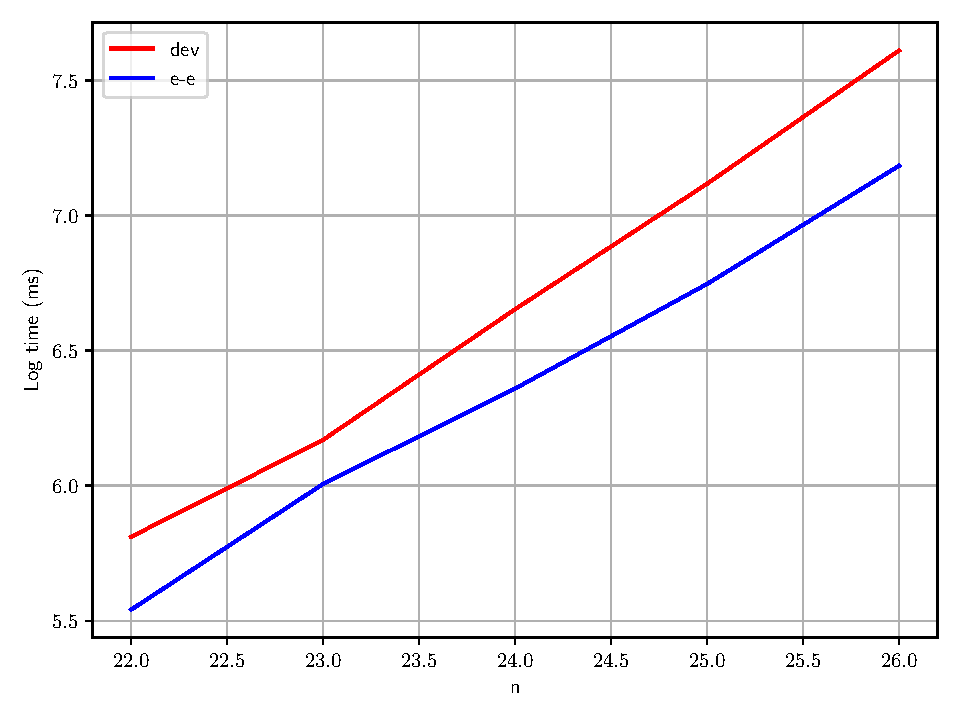
\includegraphics[width=0.7\textwidth]{img/perf_fib.pdf}
  \caption{Performance of evaluating $\text{fib}(n)$}
  \label{fig:perf-fib}
\end{figure}

\begin{figure}
  \centering
  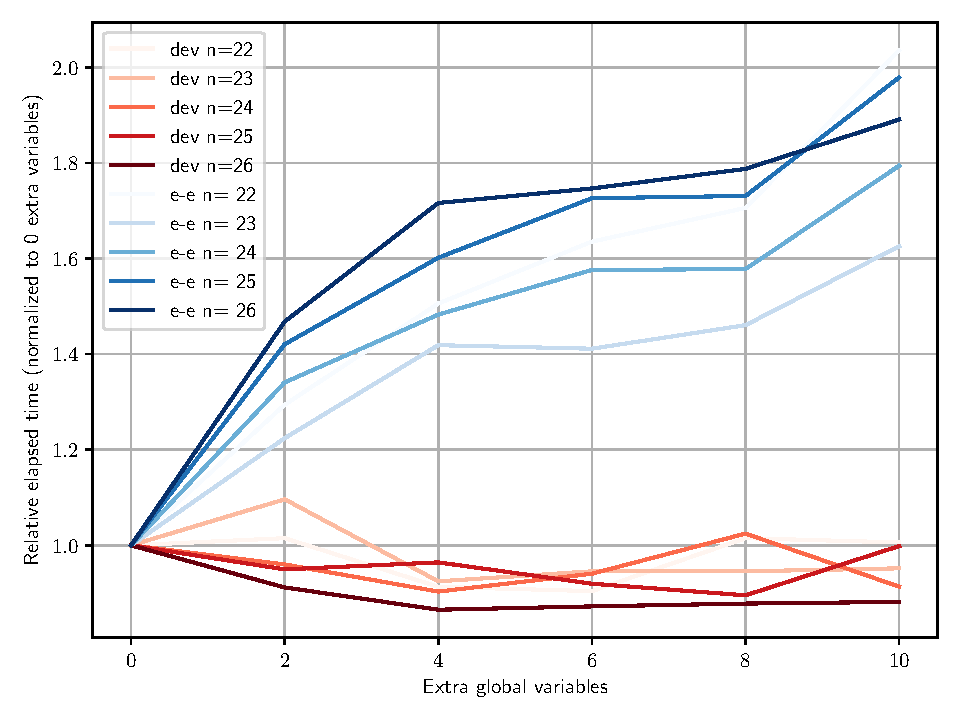
\includegraphics[width=0.7\textwidth]{img/perf_fib_more_vars.pdf}
  \caption{Performance of evaluating $\text{fib}(n)$ with extra global variables}
  \label{fig:perf-fib-more-vars}
\end{figure}

\begin{figure}
  \centering
  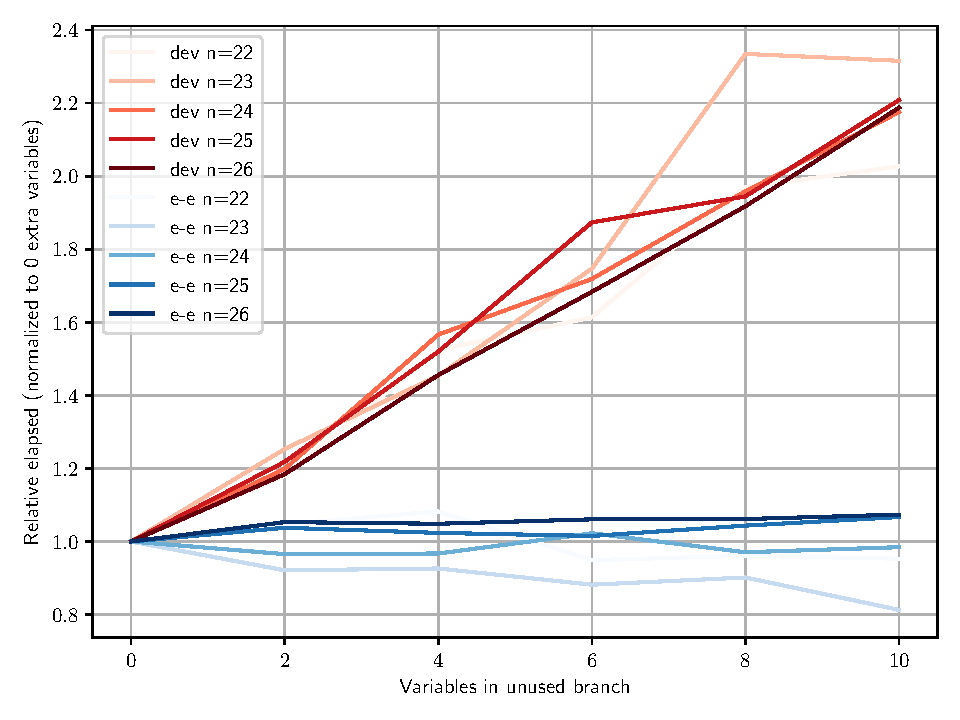
\includegraphics[width=0.7\textwidth]{img/perf_fib_more_branches.pdf}
  \caption{Performance of evaluating $\text{fib}(n)$ with an unused branch}
  \label{fig:perf-fib-more-branches}
\end{figure}


\section{Postprocessing performance}
\label{sec:evaluation-renumbering}

Consider the set of programs described by \Cref{fig:hole_renumbering_problem}.

\todo{describe this code blowup example}

\begin{singlespace}
  \begin{table}
    \centering
    \begin{tabular}{r|ccc|ccc}
      \hline
      & \multicolumn{3}{c|}{\texttt{dev} branch} & \multicolumn{3}{c}{\texttt{eval-environment} branch} \\
      & Evaluate & Postprocessing & Equality & Evaluate & Postprocessing & Equality \\
      \hline\hline
      1 & 0 & 0 & 0 & 0 & 1 & 0 \\
      2 & 0 & 0 & 0 & 0 & 1 & 0 \\
      3 & 1 & 2 & 0 & 0 & 1 & 0 \\
      4 & 1 & 1 & 1 & 1 & 0 & 0 \\
      5 & 1 & 1 & 2 & 0 & 3 & 0 \\
      6 & 5 & 1 & 3 & 1 & 0 & 0 \\
      7 & 4 & 5 & 6 & 2 & 2 & 0 \\
      8 & 3 & 3 & 14 & 0 & 0 & 0 \\
      9 & 6 & 18 & 33 & 1 & 0 & 1 \\
      10 & 14 & 29 & 61 & 0 & 0 & 0 \\
      11 & 13 & 41 & 91 & 3 & 2 & 0 \\
      12 & 25 & 145 & 203 & 2 & 0 & 1 \\
      13 & 65 & 578 & 383 & 2 & 0 & 0 \\
      14 & 147 & 2399 & 924 & 1 & 3 & 1 \\
      15 & 226 & 16597 & 1603 & 3 & 0 & 1 \\
      16 & & & & 1 & 0 & 1 \\
      17 & & & & 2 & 1 & 1 \\
      18 & & & & 0 & 3 & 1 \\
      19 & & & & 0 & 0 & 1 \\
      20 & & & & 3 & 4 & 0 \\
      21 & & & & 2 & 0 & 1 \\
      22 & & & & 0 & 2 & 1 \\
      23 & & & & 0 & 3 & 1 \\
      24 & & & & 0 & 6 & 1 \\
      25 & & & & 1 & 4 & 1 \\
      26 & & & & 1 & 2 & 1 \\
      \hline\hline
    \end{tabular}
    \caption{Performance of program illustrated in \Cref{fig:hole_renumbering_problem}}
    \label{tab:perf-hole-blowup}
  \end{table}
\end{singlespace}

\begin{figure}
  \centering
  \begin{subfigure}{0.7\textwidth}
    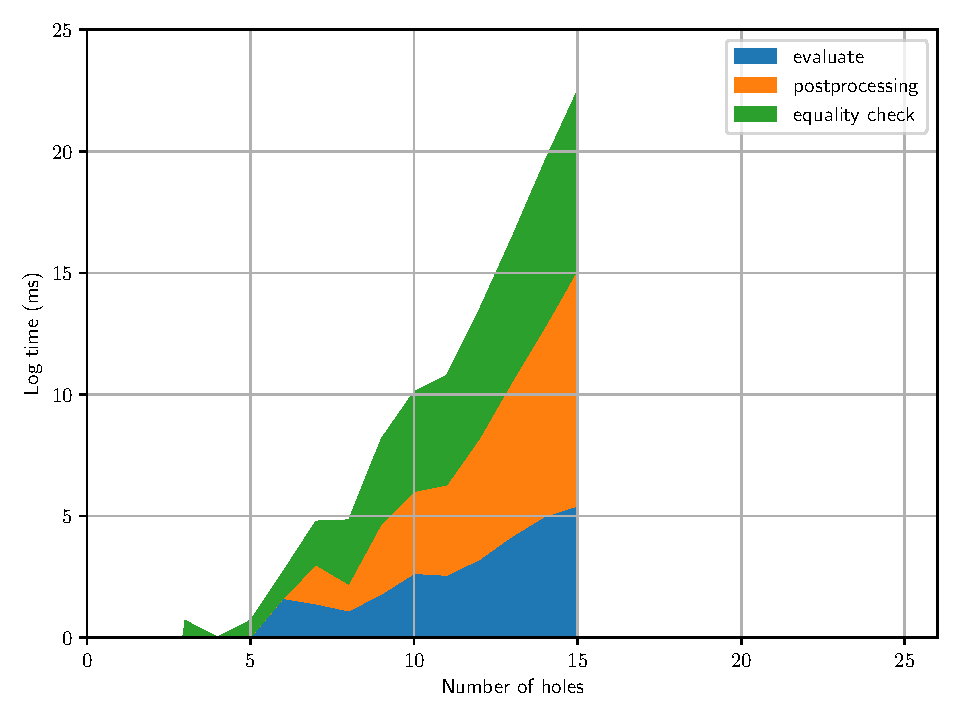
\includegraphics[width=\textwidth]{img/perf_renum_dev.pdf}
    \caption{\texttt{dev} branch}
    \label{fig:perf-renum-dev}
  \end{subfigure}
  \begin{subfigure}{0.7\textwidth}
    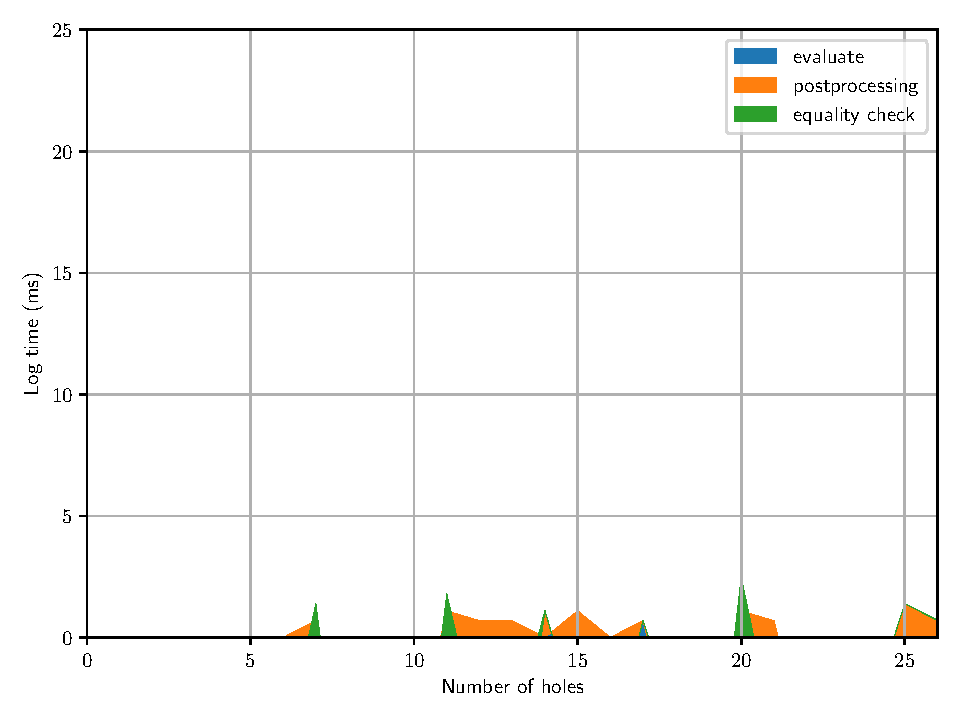
\includegraphics[width=\textwidth]{img/perf_renum_eev.pdf}
    \caption{\texttt{eval-environment} branch}
    \label{fig:perf-renum-eev}
  \end{subfigure}
  \caption{Performance of evaluating program in \Cref{fig:hole_renumbering_problem}}
  \label{fig:perf-renum}
\end{figure}

\section{FAR performance}
\label{sec:evaluation-far}

\begin{singlespace}
  \begin{table}
    \centering
    \begin{tabular}{p{10em}cccc}
      \hline
      Program & Steps & Steps & Step $\Delta$ & Cumulative \\
              & & (w/ FAR) & & Step $\Delta$ \\
      \hline\hline
      \inputhnfminted{far_fib_hist_1} & 7 & - & 0 & 0 \\ \hline
      \inputhnfminted{far_fib_hist_2} & 12 & 21 & 9 & 9 \\ \hline
      \inputhnfminted{far_fib_hist_3} & 17 & - & 0 & 9 \\ \hline
      \inputhnfminted{far_fib_hist_4} & 58 & 69 & 11 & 20 \\ \hline
      \inputhnfminted{far_fib_hist_5} & 4762964 & - & 0 & 20 \\ \hline
      \inputhnfminted{far_fib_hist_6} & 4762966 & 12 & -4762954 & -4762934 \\ \hline
      \inputhnfminted{far_fib_hist_7} & 4762966 & 21 & -4762954 & -9525879 \\ \hline
      \inputhnfminted{far_fib_hist_8} & 4792967 & 13 & -4792954 & -14288813 \\ \hline
      \hline
    \end{tabular}
    \caption{A program edit history with an expensive computation}
    \label{fig:far-program-history-fib}
  \end{table}
\end{singlespace}

\begin{singlespace}
  \begin{table}
    \centering
    \begin{tabular}{p{10em}cccc}
      \hline
      Program & Steps & Steps & Step $\Delta$ & Cumulative \\
              & & (w/ FAR) & & Step $\Delta$ \\
      \hline\hline
      \inputhnfminted{far_hist_1} & 1 & - & 0 & 0 \\ \hline
      \inputhnfminted{far_hist_2} & 2 & 3 & 1 & 1 \\ \hline
      \inputhnfminted{far_hist_3} & 3 & - & 0 & 1 \\ \hline
      \inputhnfminted{far_hist_4} & 4 & 5 & 1 & 2 \\ \hline
      \inputhnfminted{far_hist_5} & 5 & - & 0 & 2 \\ \hline
      \inputhnfminted{far_hist_6} & 6 & 9 & 3 & 5 \\ \hline
      \inputhnfminted{far_hist_7} & 8 & 8 & 0 & 5 \\ \hline
      \inputhnfminted{far_hist_8} & 9 & 14 & 5 & 10 \\ \hline
      \inputhnfminted{far_hist_9} & 10 & 11 & 1 & 11 \\ \hline
      \inputhnfminted{far_hist_10} & 11 & 6 & -5 & 6 \\ \hline
      \hline
    \end{tabular}
    \caption{A sample edit history for a simple program}
    \label{fig:far-program-history-simple}
  \end{table}
\end{singlespace}

\begin{figure}
  \centering
  \begin{subfigure}{0.7\textwidth}
    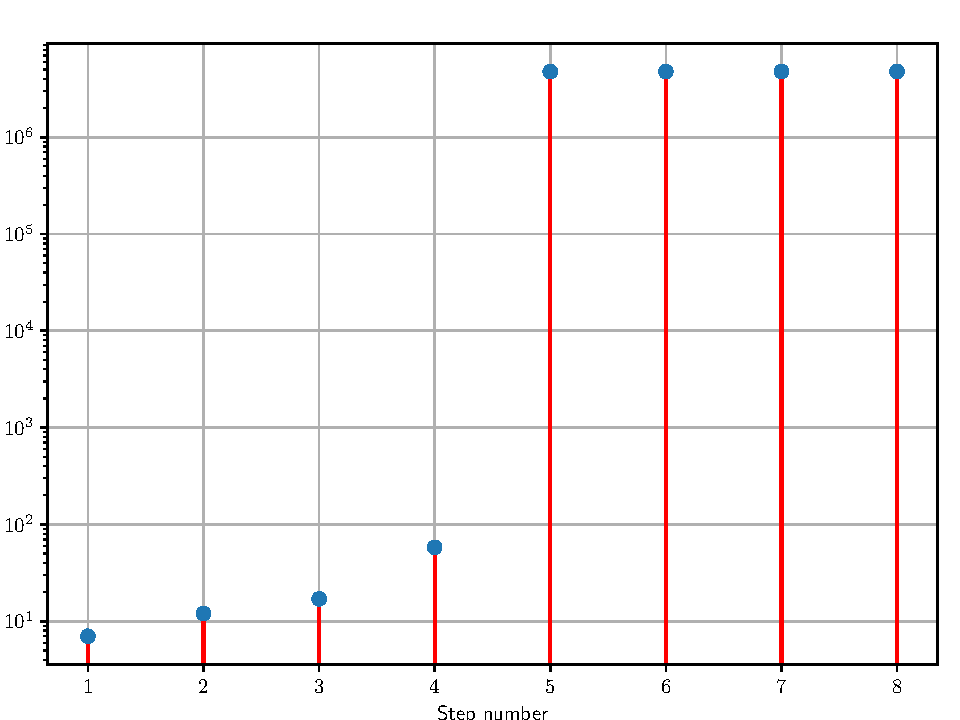
\includegraphics[width=\textwidth]{img/perf_no_far.pdf}
    \caption{Normal evaluation}
    \label{fig:perf-no-far}
  \end{subfigure}
  \begin{subfigure}{0.7\textwidth}
    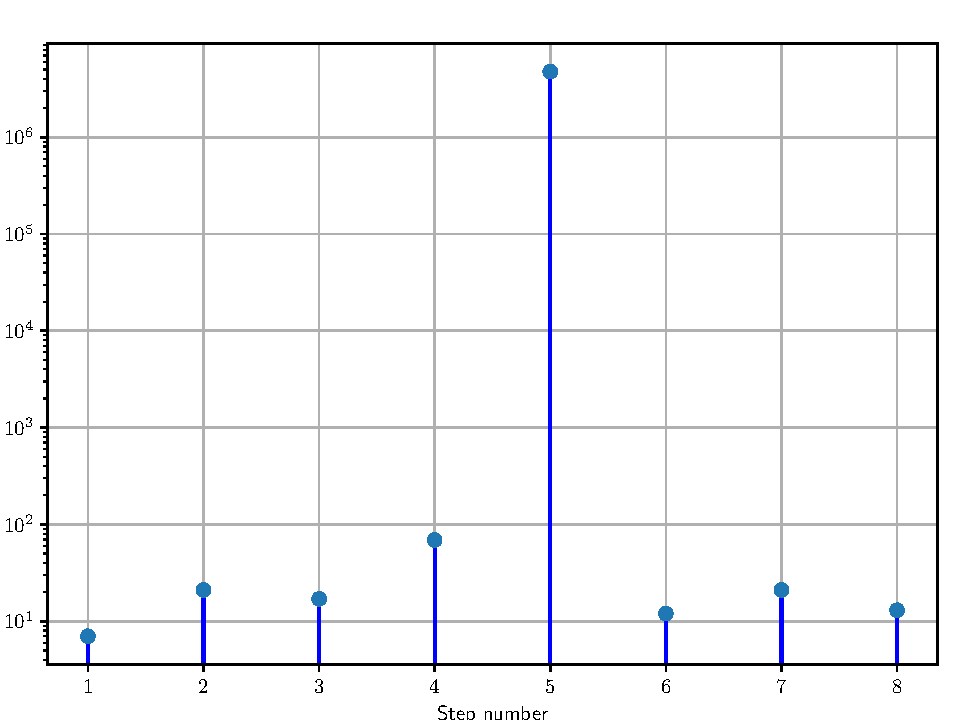
\includegraphics[width=\textwidth]{img/perf_far.pdf}
    \caption{With one-step FAR}
    \label{fig:perf-far-far}
  \end{subfigure}
  \caption{Number of evaluation steps per edit in \Cref{fig:far-program-history-fib}}
  \label{fig:perf-far}
\end{figure}

%%% Local Variables:
%%% mode: latex
%%% TeX-master: "main"
%%% End:

\chapter{Conclusions and recommendations}
\label{sec:concl}

This thesis explores several advancements to the evaluation model in Hazel, an implementation of a live programming editor with typed holes. We develop rules and a metatheory for the propesd changes as well as a working implementation for most of the rules provided.

The first proposed change is the switch from using variable substitution at binding time to storing variables in an environment at lookup time. This implementation leads to the introduction of closures to the internal language of Hazel, as well as a postprocessing step to restore the same result that would have been achieved by evaluation using the substitution model. Initially, we begin with the conventional function closures and the hole closures introduced in Hazelnut. Later, we introduce generalized closures, which subsume function and hole closures, and represent any paused evaluation. Generalized closures play a critical role in FAR.

The second major change is the use of the environment model to memoize operations that occur on shared environments. Environments are uniquely numbered to allow for lookup and memoization. Memoization is applied to the hole renumbering process (in the process changing the useful interpretation from hole instances to hole closures), and to speed up the structural equality checking. Memoization may also be helpful with the re-evaluation with filled expressions and environments during the FAR re-evaluation process, but this has not been fully implemented yet.

The third major contribution is a set of practical considerations to implementing the fill-and-resume (FAR) optimization, as originally proposed in Hazelnut Live. FAR promotes resuming evaluation from a previous evaluation result when an edit action is performed, as opposed to restarting evaluation from the beginning on every edit action.  Firstly, we describe a structural diffing algorithm for detection of a valid fill operation. This algorithm is intuitive and robust to work between an arbitrary past edit state and the current edit state (a $n$-step fill operation). We also provide the basic semantics for the fill (preprocessing) and resume (re-evaluation) operations. A 1-step FAR operation is implemented as a proof of concept.

We evaluate the performance of these methods empirically, via a series of benchmarks of sample programs. We compare the difference between the current main development branch on the \texttt{dev} branch to an updated evaluation model implementing the changes proposed in this thesis, in the \texttt{eval-environment} and \texttt{fill-and-resume-backend} branches. The results qualitatively match the expectation. Evaluation with environments is beneficial for performance when lazy variable lookups are reduced and the environment size is small. Substitution may be beneficial for performance when the number of substitution passes is small. The memoization of environments solves the performance issue in the program that motivated the memoization of environments in the hole numbering and structural equality checking processes. FAR provides a great improvement in efficiency when there is a valid fill operation and expensive re-computations can be avoided. However, FAR may sometimes be more expensive than regular evaluation from the beginning, due to the recursive re-evaluation of environments. Future work on this environment memoization and the implementation of the $n$-step fill operation should further improve the performance benefit of FAR.

We do not prove the correctness of the implementation. We instead provide a metatheory governing the implementation and provide a logical intuition for the correctness of the proposed metatheorems. We leave formal proofs of the metatheory and proofs of the completenes of the metatheorems to future work.

The primary goal of this work is to inform future development on Hazel or related research efforts, and the explanations and motivations have been written in enough detail to allow for others to independently reproduce this work. The implementation of the rules in this work are intended to act as a reference implementation and not necessarily be incorporated directly into the main development branches; the theoretical discussion is the more useful part of this work. We discuss practical tradeoffs of implementing evaluation with environments. Evaluation using environments leads to some improvement in performance in many programs where lazy variable lookup is beneficial, and leads to a major improvement in performance in some programs due to the effect of memoizing environments, but comes at the expense of a great deal of extra complexity that may obscure Hazel's original goal in approaching the gap problem. We also describe a possible implementation of FAR and entrypoint for the FAR algorithm, with possibilities for further memoizing re-evaluation. The empirical results that are presented may serves as a guideline for performance benefits, but it will be useful to collect user editing and program statistics to better evaluate the average or expected performance benefit of the proposed changes. Along the way, we introduce several novel generalizations that both simplify implementation and give nice theoretical interpretations, such as generalized closures and the presentation of $n$-step FAR as a generalization of evaluation.

%%% Local Variables:
%%% mode: latex
%%% TeX-master: "main"
%%% End:


% bibliography
\clearpage{}
\addcontentsline{toc}{section}{References}
\pt{References}
\bibliography{refs}

% appendices
\clearpage{}
\appendix{}
\addcontentsline{toc}{section}{Appendices}
\pt{Appendices}
% TODO: put this header on the same page as the first appendix

\section{Formalization of evaluation with environments}
\label{app:eval_env}

%%% Local Variables:
%%% mode: latex
%%% TeX-master: "main"
%%% End:

\chapter{Additional contributions to Hazel}
\label{app:contributions}

\section{Additional performance improvements}
\label{sec:other_perf}

% fast structural equality checking w/ environments
% remove multiple calls to Program.get_result

\section{Documentation and learning efforts}
\label{sec:study_group}

% study/reading group
% documentation: module-level and visual overview

%%% Local Variables:
%%% mode: latex
%%% TeX-master: "main"
%%% End:

\section{Selected code samples}
\label{app:code_samples}

%%% Local Variables:
%%% mode: latex
%%% TeX-master: "main"
%%% End:


\end{document}

%%% Local Variables:
%%% mode: latex
%%% TeX-master: t
%%% End:
